\chapter{Circuit and PCB design}
%
Using the results from the last section the circuit for the individual modules is designed.
%
\section{DAC}

\begin{enumerate}
  \item Requirements
  \subitem >= 120ks/s
  \subitem Fast enough digital interface
  \subsubitem package size * samplingrate
  \subitem Handsolder SMD package
  \subitem 5V VCC
  \item component/model decision
  \item I2C vs. SPI
  \item pcb layout
\end{enumerate}

\Gls{CASA}
\Gls{CMF}
\section{Ultrasonic Transducers}

The ultrasonic transducer chosen for this project is the CUSA-T80-15-2400-TH. It has an operating frequency of $40kHz$ and tolerates a supply voltage up to $80V$.\cite{cui_devices_cusa-t80-15-2400-th_2020}\newpage
\noindent One module uses $19$ transducers which are connected in parallel as shown in figure \ref{fig:pcb:transducer_circuit}. In order to create the aspired beamforming effect the transducers are evenly distributed on the pcb (figure \ref{fig:pcb:front}).
%
\begin{figure}
  \centering
  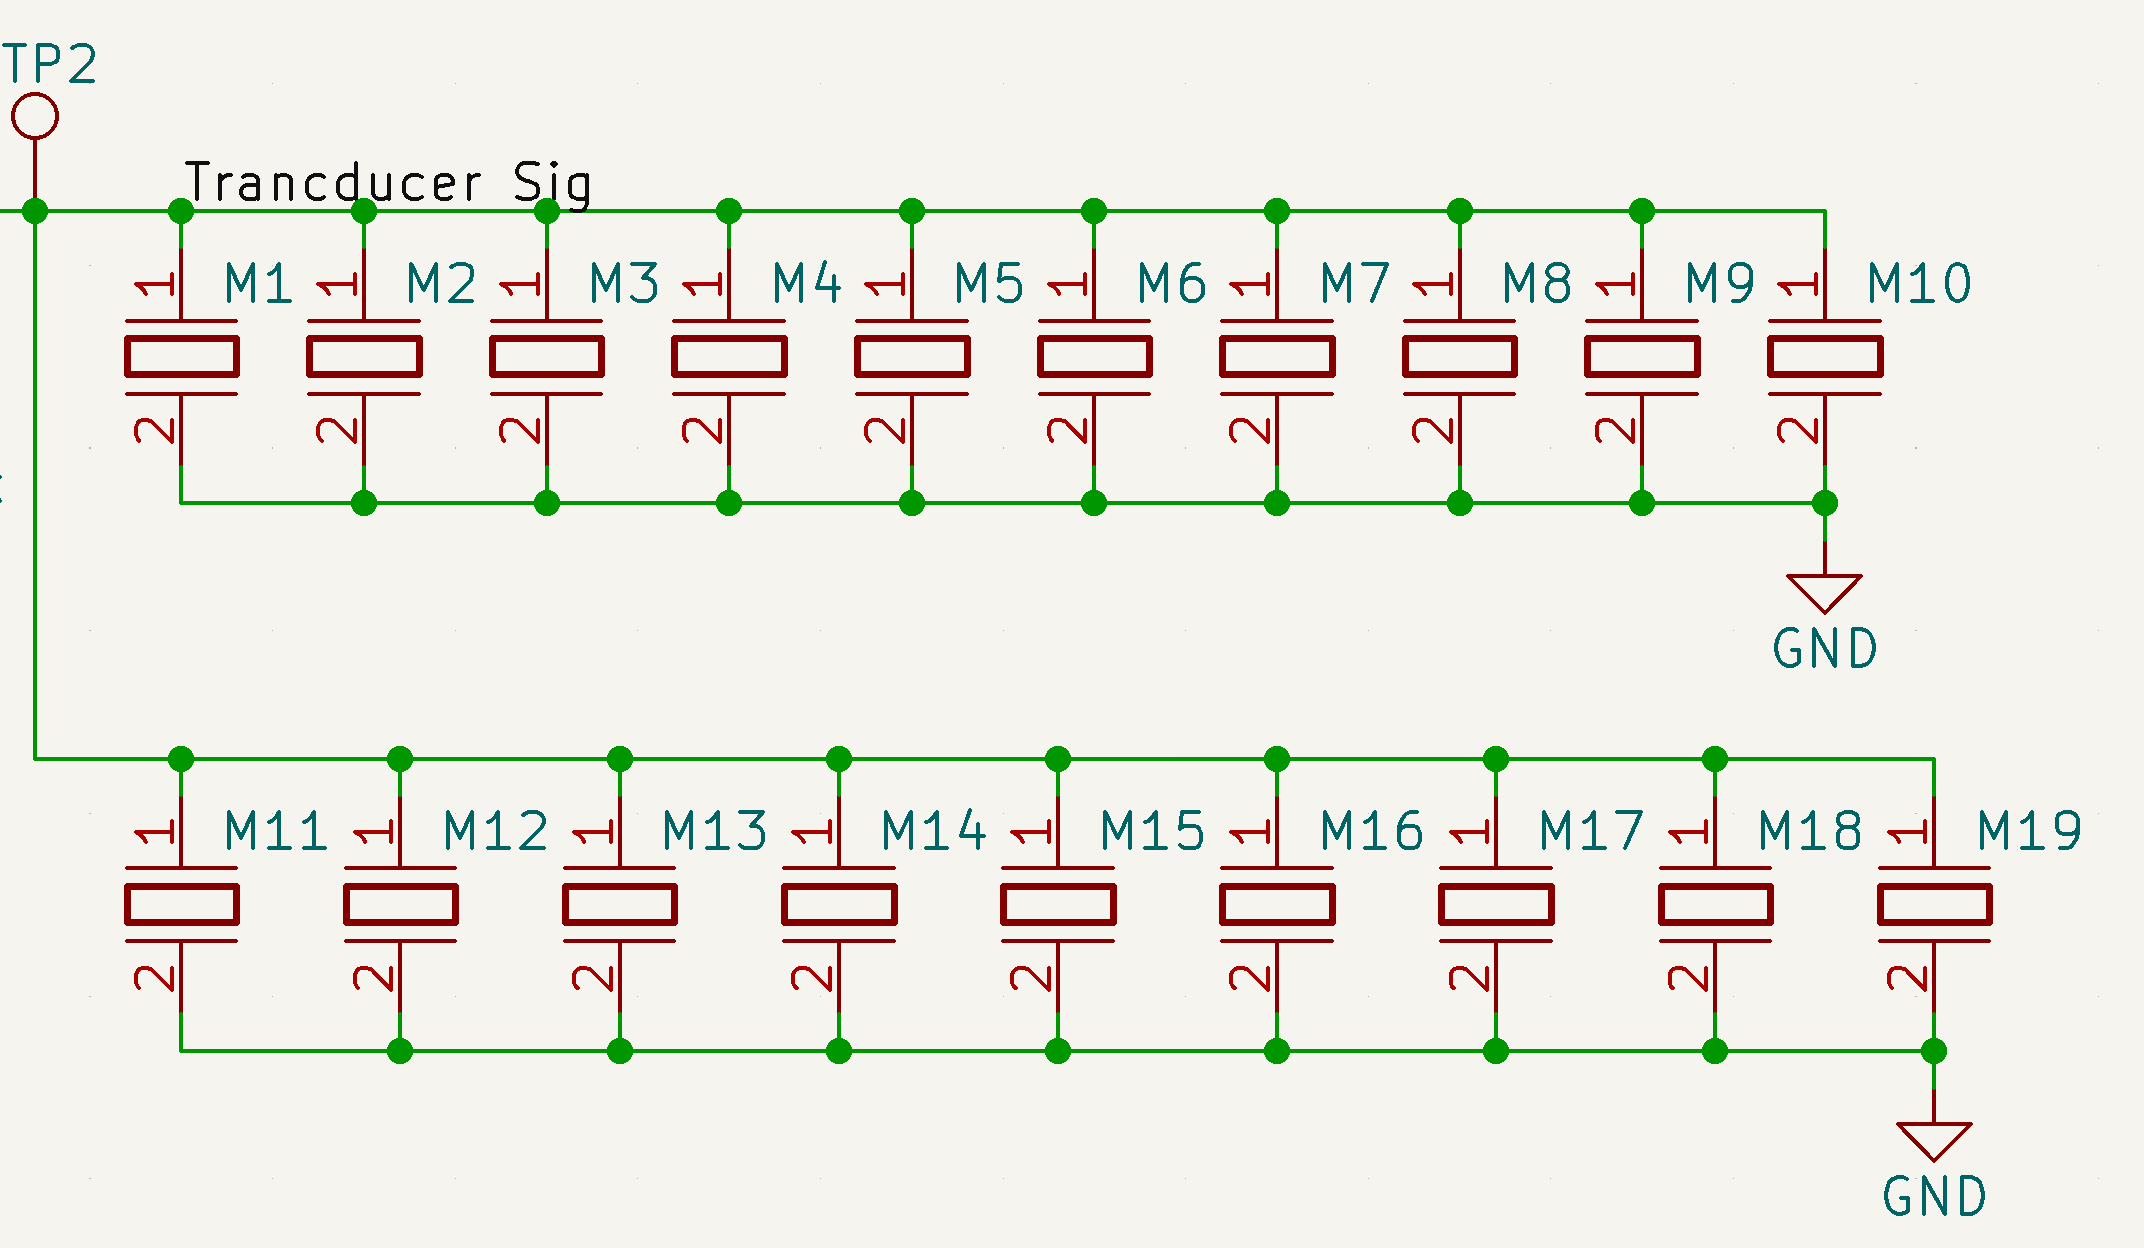
\includegraphics[height=\mediumheight]{src/assets/pictures/circuit/transducer_circuit.png}
  \caption{Transducer circuit design}\label{fig:pcb:transducer_circuit}
\end{figure}
\section{Amplifier}\label{sec:pcb:amp}

\begin{enumerate}
  \item Requirements
  \subitem VCC >= 24V -> Why
  \item pcb layout
\end{enumerate}

Ultrasonic transducer have to be driven with a much higher voltage and current than a DAC can provide. Therefore an amplifier circuit was designed wich takes the DAC voltage as input and generates a suitable output for the array of ultrasonic transducers.

\subsection{Circuit}

The amplifier consists of two sections. First a non-inverting amplifier circuit to amplify the input voltage. Next a Class B power amplifier is used so the circuit is able to drive the high capacitive load of the transducers. The whole circuit is designed for single supply because the powersupply only provides a positive voltage.\p

\subsubsection*{Voltage input}
%
\comp{C8} is used to filter the DC part of the inputsignal. \comp{R8} and \comp{R9} then generate a new operating point at $12V$. For AC signals a DC power supply can be seen as short circuit. This will result in \comp{R8} and \comp{R9} being parallel (Figure \dots). Combined with \comp{C8} they build a simple high pass wich can be calculated for a specific cut-off frequency.
%
\begin{align}
  R_8 || R_9 &= \frac{1}{2} R_{8/9} \pmath
  \cfrac{U_a}{U_{in}} &= \cfrac{sC_8\cdot \frac{1}{2}R_{R8/9}}{1 + sC_8\cdot \frac{1}{2}R_{8/9}} \pmath
  f_g &= \cfrac{1}{2 \pi C_8 \cdot \frac{1}{2}R_{R8/9}} \pmath
  C_8 &= \cfrac{1}{2 \pi f_g \cdot \frac{1}{2}R_{R8/9}}
\end{align}
%
As cut-off frequency $4kHz$ was chosen and for \comp{R8} and \comp{R9} a value of $100k\Omega$ was selected. This results in a capacity of around $1.5nF$ for \comp{C8}.

\subsubsection*{Feedback}
%
Because of the new operating point of the input only AC signals should be amplified by the OpAmp. This is achieved with the capacity \comp{C9} in the feedback. The capacity blocks signals below the cut-off frequency creating a voltage follower. For signals above the cut-off frequency the capacity acts as a short circuit. The transfer function of the feedback can be used to calculate \comp{C9}. A capacitance of $10nF$ was selected. This results in a cut-off frequency of around $3.2kHz$.
%
\begin{align}
  A &= \frac{1 + s C_9 (R_3 + R_4)}{1 + s C_9 R_4}\pmath
  f_g &= \frac{1}{2 \pi C_9 R_4}
\end{align}
%
The amplification can be calculated like a non-inverting amplifier. In order to take advantage of the $24V$ voltage range with the $4V$ DAC output (At this point it was not clear, that this version of the DAC would not be available) the amplification should be $4$. With $R_3 = 15k\Omega$ this results in a \comp{R4} of around $5.1k\Omega$.
%
\begin{align}
  V = 1 + \frac{R_3}{R_4}
\end{align}
%
\subsubsection*{Voltage output}
At the output of the circuit a highpass filter is used to filter the $12V$ DC voltage caused by the voltage divider at the input.

\begin{align}
  A &= \cfrac{sC_{10} \cdot Z_{10}}{1 + sC_{10} \cdot Z_{10}} \pmath
  f_g &= \frac{1}{2 \pi C_{10} \cdot Z_{10}}
  Z_{10} = R_{10} || Z_M
\end{align}
%
Because the behaviour of this highpass depends on the $ESR$ and capacity of all transducers, the size of \comp{C10} was determined empirically. The best results where achieved with $10uF$.

\subsection{Stability}

As described above a power amplifier is needed to drive the high current of the ultrasonic transducers. A class B amplifier was chosen because of its simple but powerefficient design. Usually this design causes crossover distortion. This is solved by putting the feedback behind the power amplifier.\p
%
\textbf{REWORK}\p
Using this solution opens another set of problems. To improve stability OpAmps are usually phase compensated to represent a first order lowpass. This is now disturbed by the power amplifier.\p
%
In order to verify the stability the frequency response of the circuit was measured.\p
\textbf{REWORK}\p
%
Note that this is only possible if the OpAmp is powerfull enough to drive the base current of the transistors. A better solution for higher currents would be to use the more complex class AB power amplifier.\p
\section{Powersupply}
%
\begin{figure}[ht]
  \begin{subfigure}[b]{0.49\textwidth}
    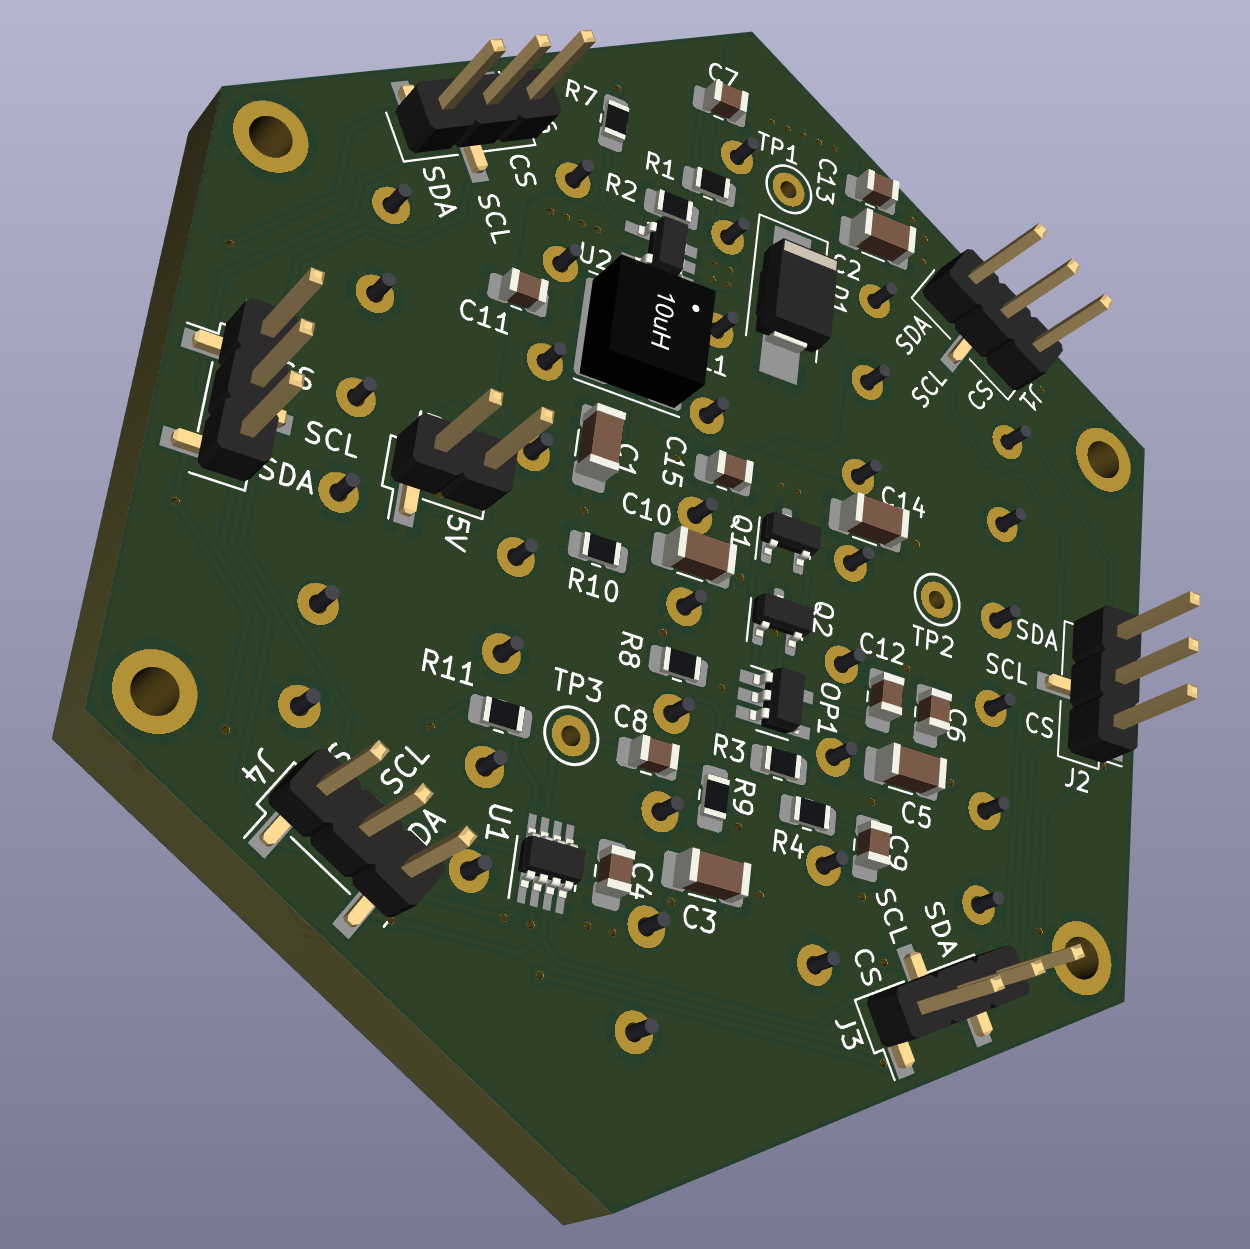
\includegraphics[width=\textwidth]{src/assets/pictures/circuit/pcb_back.png}
    \caption{Back}
    \label{fig:pcb:back}
  \end{subfigure}
  \hfill
  \begin{subfigure}[b]{0.49\textwidth}
    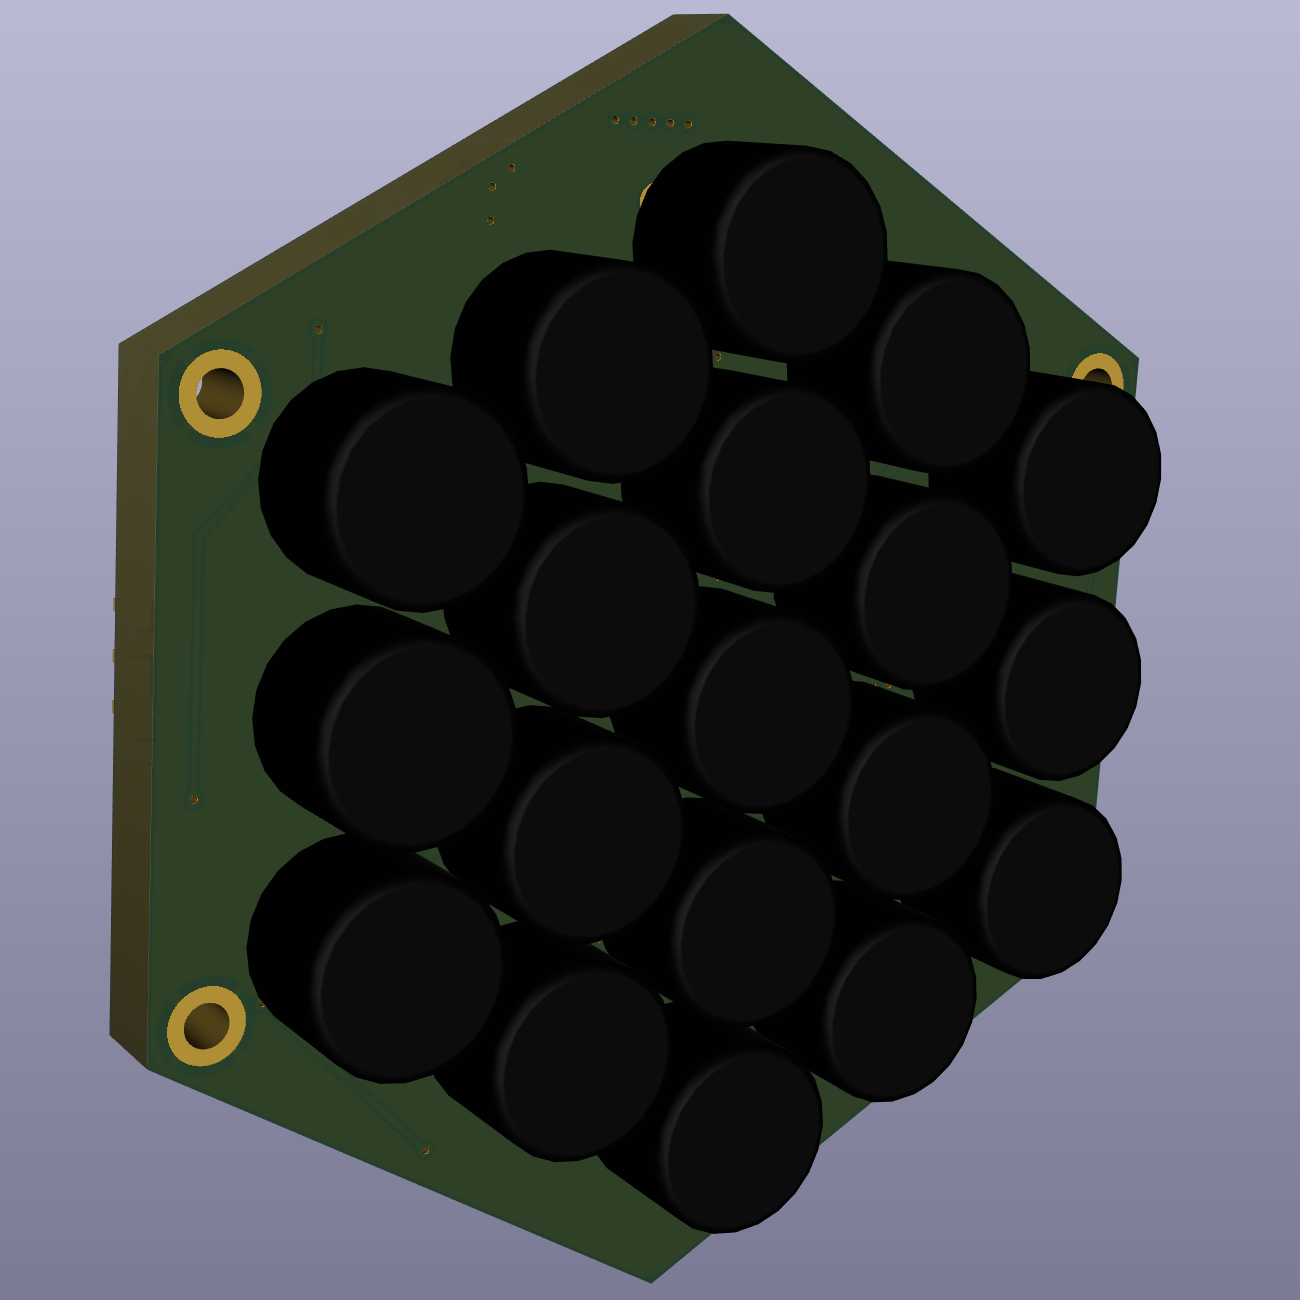
\includegraphics[width=\textwidth]{src/assets/pictures/circuit/pcb_front.png}
    \caption{Front}
    \label{fig:pcb:front}
  \end{subfigure}
  \caption{3D model of the PCB layout}
  \label{fig:pcb}
\end{figure}
%